% this file is called up by thesis.tex
% content in this file will be fed into the main document

\chapter{Design} % top level followed by section, subsection

\section{A Case for CSx Emulation}

\label{emulatecase}

The lack of a standardized design has lead to a large variety of different
hardware architectures being explored including using embedded CPUs or
\textit{Field-Programmable Gate Arrays} (FPGA)s. Moreover, closed-source
devices have even become commercially available. Still there is a lot of
uncertainty about the right computational hardware models, interconnects and
interconnects their interfaces \cite{barbalacecomputational}. In addition,
the engineering of hardware is significant and domain specific limiting the 
design space exploration that can be achieved \cite{10.1145/3439839.3459085}.
Currently, the \textit{Peripheral Component Interconnect Express} (PCIe)
interconnect and the NVMe storage interface currently dominate modern storage
devices. However, it is unclear if their current capabilities are sufficient to
support CSxs. Meanwhile existing technologies such as QEMU allow rapid
development of new simulated hardware.

The lack of a clear standardized design combined with the ease of prototyping
designs in emulation clearly shows that choosing emulation over an actual
hardware prototype is the current logical choice.

\section{A Case for eBPF Programmability}

\label{ebpfcase}

The concept of programmability provides end users the capability to run their
own provided code. With the introduction of modern \textit{Operating Systems}
(OS)s this is expected to happen in safe and dynamic manner. Programmability
can be achieved in different manners such as through the kernel in kernel
modules, with filesystems through \textit{Virtual FileSystem} (VFS) \cite{vfs}
or \textit{Filesystem in USErspace} (FUSE) \cite{fuse} and with language
runtimes such as those in Python. In addition programmability can also target a
peripherals instead of the host directly such as is prevalent in
\textit{General-Purpose computing on Graphics Processing Units} (GPGPU)
programming through \textit{Application Programming Interfaces} (API)s like
OpenCL \cite{opencl} and CUDA \cite{cuda}. Through similar mechanisms
programmability in CSxs can be achieved.

The uncertainty of the hardware design makes it unclear exactly how close to the
hardware and through which method of programmability CSxs will be effective.
Although, naturally, the closer to the actual storage the better
(Near-Data Processing). Therefore, our programmability must not be restricted or
favor a particular type.

Introducing eBPF an ISA and \textit{Application Binary Interface} (ABI) with a
large collection of toolchains and wide-ranging implementations
\cite{what-ebpf, McCanne1993TheBP}. Among these implementations is XRP which
uses eBPF to increase storage performance by mitigating part of the Linux kernel
storage stack \cite{280870}. Furthermore, these implementations range from
complex, such as the one found in the Linux kernel, to simple such as the one
found in uBPF \cite{ubpf}, with the key difference in complexity being the
supported ABI. Effectively, the implementation running (runtime) eBPF code
decides the ABI by tying special eBPF (sys)call instructions to predefined code.
In addition, this allows the user program and runtime to exchange important
information such as prominently done in Linux through eBPF maps \cite{bpf-man}.
We demonstrate the flexibility of such a vendor agnostic ABI as well as the
internals of uBPF in figure \ref{figure:ubpf-abi}.

\begin{figure}
    \centering
	\includegraphics[width=0.8\textwidth]{resources/images/ubpf-abi.pdf}
	\caption{Achieving vendor agnostic \textit{Application Binary Interfaces}
        (ABI) through uBPF.}
    % \includesvg[width=0.6\columnwidth]{resources/images/module-dependencies}
    \label{figure:ubpf-abi}
\end{figure}

The benefits of eBPF are four fold. First, the ISA is not tailored to any
specific domain and it has been used in networking \cite{xdp},
tracing \cite{enhanced-ebpf}, security \cite{seccomp} and storage \cite{280870}
applications. Second, the simple nature of the eBPF ISA allows for verification
and bounded execution checking such as performed by the Linux kernel
\cite{kern-analysis}. Third, eBPF supports efficient code generation through
jitting (Just in Time compilation) achieving close to bare-metal performance.
Lastly, eBPF has been positioned as the unified ISA for heterogeneous computing
\cite{Brunella2020hXDPES, bpf-uapi}.

\section{A Case for ZNS}

\label{znscase}

A new emerging NVMe standard is \textit{Zoned NameSpaces} (ZNS) \cite{zns}. It
can been seen as the technical successor to Open-Channel
\cite{Bjrling2017LightNVMTL}. This standard allows host visibility and control
over data placement (host-managed) while more closely representing NAND flash
behaviour. This replacement for the traditional block interface offers reduced
write-amplification, lower SSD hardware requirements and more intelligent
wear-levelling and garbage collection. In addition, the better control
allows for higher throughput and reduced tail latency \cite{273945}. However,
ZNS SSDs come with several constraints such as not allowing in-place updates
(append only), using a large collection of sectors as single erasure unit and
requiring wear-levelling and garbage collection to be explicitly programmed by
the host. The fundamental difference between conventional and ZNS SSDs is shown
in figure \ref{figure:znsvsconventional}.

\begin{figure}
    \centering
	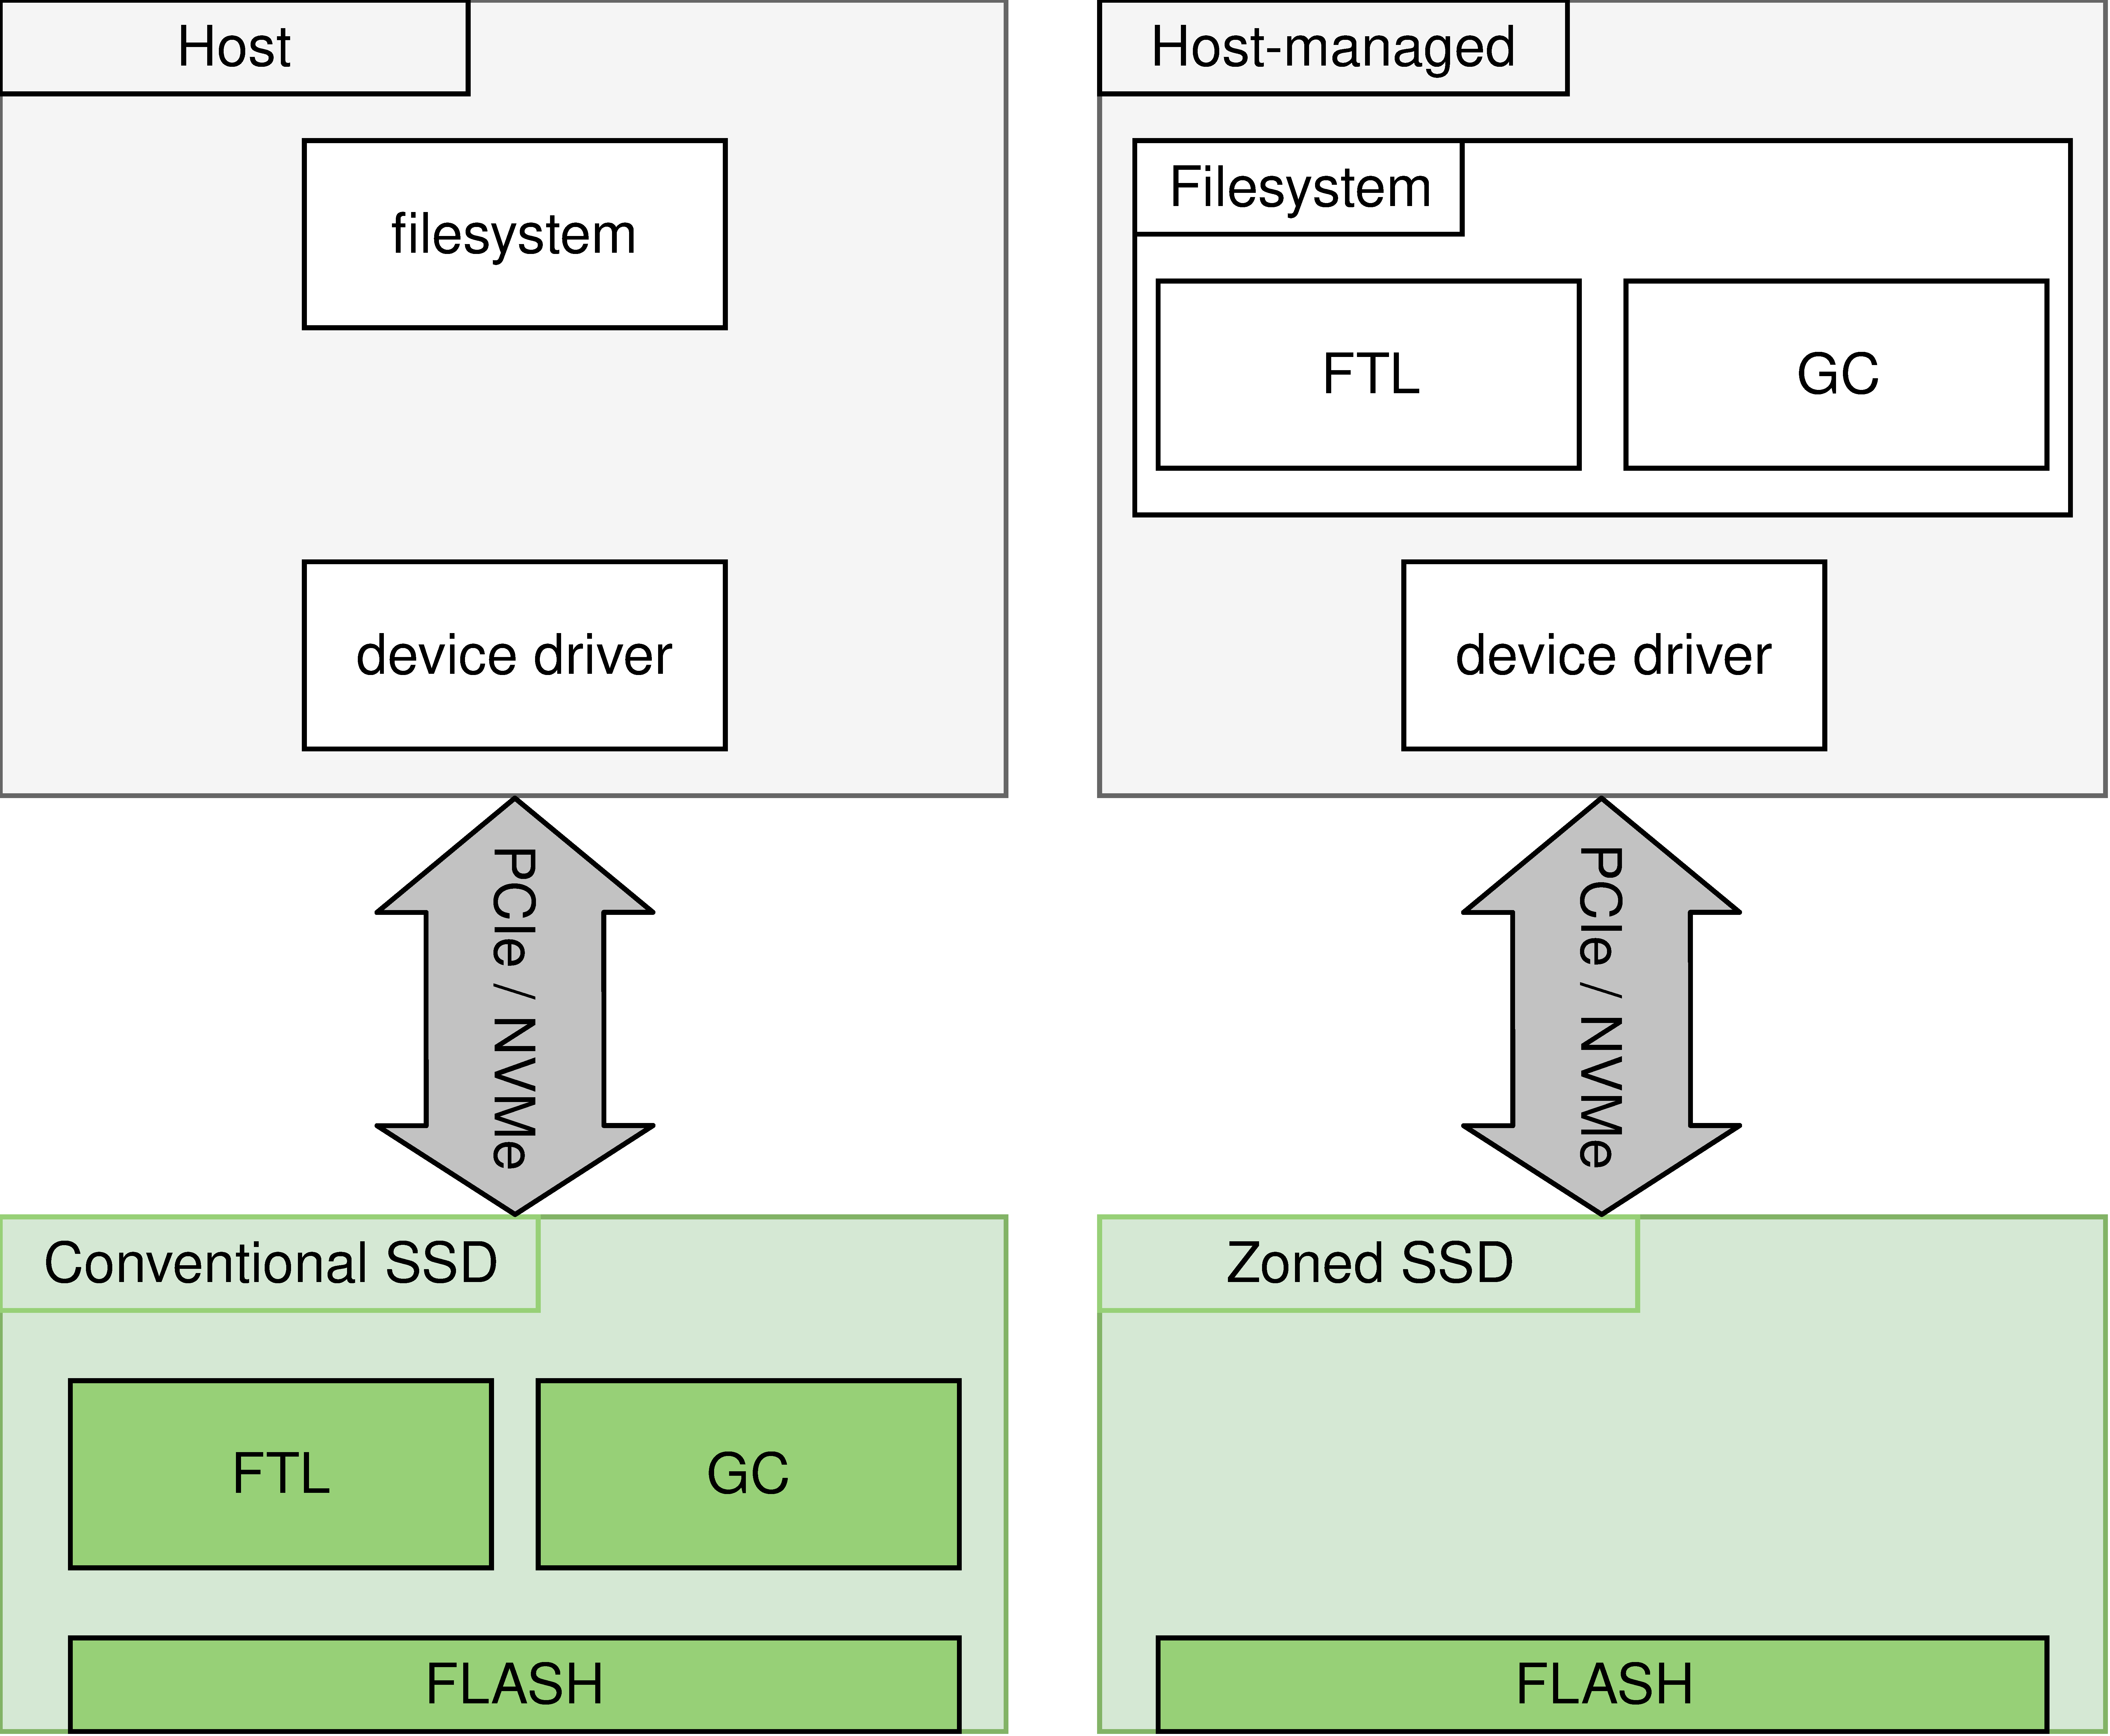
\includegraphics[width=0.6\textwidth]{resources/images/zns-vs-conventional.pdf}
	\caption{Differences between conventional and ZNS SSDs.}
    % \includesvg[width=0.6\columnwidth]{resources/images/module-dependencies}
    \label{figure:znsvsconventional}
\end{figure}

Yet we argue ZNS greatly improves the feasibility of CSxs supporting
\textit{hybrid filesystems}. Firstly, ZNS offers more predictable performance in
conjunction with \textit{Log-Structured Filesystems} as the absence of a device
FTL means the behaviour of \textit{append-only} writes will not be influenced by
underlying write-amplification or garbage-collection. Secondly, the direct
relationship between dimensions as reported to the host and to those known on
the device results in a greatly simplified exchange of information from host
submitted compute kernels as well as reduced kernel runtime translations.
Finally, this reduced semantic gap between the host and device is essential for
compute kernels running autonomously and without shared virtual memory.

\section{A Case for LFS}

\label{lfscase}

\textit{Log-Structured Filesystems} have been around for a long
time \cite{Rosenblum1992TheDA} but have not really been popularized until the
recent advancement of NAND flash. A LFS maintains one or multiple logs which
are append only sections of the filesystem. This has the advantage of the
underlying device receiving filesystem writes as sequential I/O operations,
which is known to improve performance. In addition, LFSs are often relatively
easy to implement. Unfortunately, LFSs suffer from write-amplification because
modifications updating inode or other data location information travels up the
chain in history. The specific type of write-amplification common in LFSs is
also known as the wandering tree problem. An example of write-amplification is
shown in figure \ref{figure:writeamplification}.

\begin{figure}
    \centering
	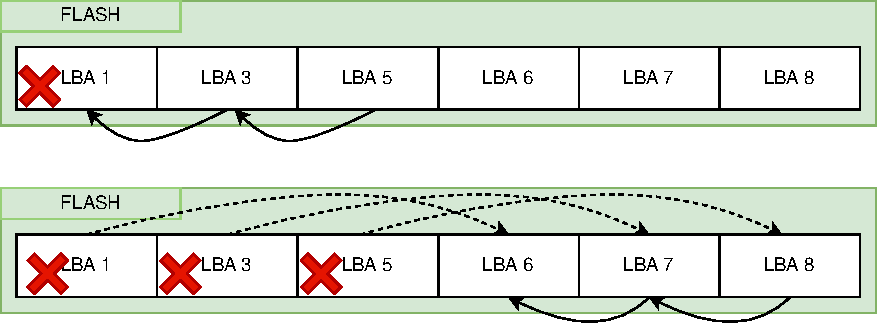
\includegraphics[width=0.7\textwidth]{resources/images/write-amplification.pdf}
	\caption{Example of write-amplification where a single invalidation leads
    to multiple linked blocks being rewritten.}
    % \includesvg[width=0.6\columnwidth]{resources/images/module-dependencies}
    \label{figure:writeamplification}
\end{figure}

Yet we argue an LFS is essential for an effective \textit{hybrid filesystem} due
to the following three reasons. Firstly, the append-only nature of a LFS is the
best fit for the append-only requirement of ZNS SSDs. Secondly, the
chronological order of logs allows for snapshotting, versioning and simplified
crash recovery. It is thanks to the properties of an LFS that FluffleFS is able
to provide in-memory snapshots to compute kernels. Lastly, the problem around
write-amplification is a solved issue thanks to the work of F2FS
\cite{Lee2015F2FSAN} which introduced a so called \textit{Node Address Table}
(NAT). A diagram showing a simplified view of F2FS and the NAT is shown in
figure \ref{figure:f2fsnat}.

\begin{figure}
    \centering
	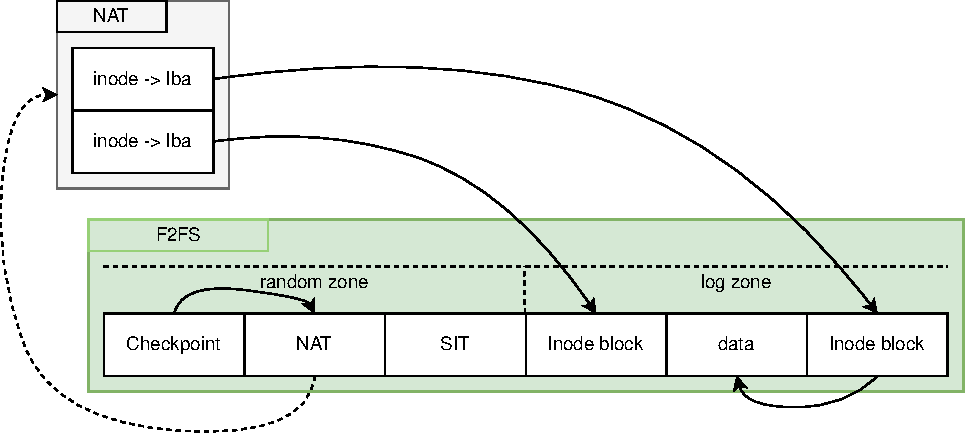
\includegraphics[width=0.7\textwidth]{resources/images/f2fs-nat.pdf}
	\caption{Overcoming LFS limitations with a separate random zone and NAT.}
    % \includesvg[width=0.6\columnwidth]{resources/images/module-dependencies}
    \label{figure:f2fsnat}
\end{figure}

As shown each of these cases demonstrates the importance of each part. Only
together are they able to provide a complete solution for open research
questions given the current state of the field as we will proof in the design
section.

\section{Requirements}

As mentioned our research questions are divided to address both design and
evaluation separately. In addition, the design requirements can be further
divided into those addressing the overall filesystem, the surrounding
framework and computational offloading. The resulting categorization is shown
below.

\begin{itemize}
    \item Framework
    \begin{enumerate}
        \item What techniques can be used to minimize the complexity required to
            use a hybrid LFS?
        \item What mechanisms allow for simplified replacement of used existing
            technologies in a hybrid LFS?
    \end{enumerate}
    \item Filesystem
    \begin{enumerate}
        \item What existing technologies are best suited for a hybrid LFS?
    \end{enumerate}
    \item Offloading
    \begin{enumerate}
        \item How to register CSx compute kernels using existing operating
            system APIs?
        \item How to differentiate individual users, files and I/O operations in
            relation to their CSx compute kernel?
        \item How to design a compute kernel API that can be reused across devices?
        \item How to ensure user submitted CSx compute kernels are safe?
    \end{enumerate}
\end{itemize}

\subsection{Framework}

Traditional CSx prototypes often have a high barrier to entree due to
complicated dependencies that can not easily be installed through package
managers or software repositories. Our work directly addresses that minimizing
the complexity as design requirement as well as designing for simple
replacement of used technologies.

Firstly, all software dependencies must be installed isolated from system
dependencies. This is to prevent the host system being influenced by the use
of the prototype. Secondly, as many as possible software dependencies must be
userspace programs such that even users without administrative system
privileges can use it. Finally, the prototype must be able to run in a virtual
environment that allows for the emulation of ZNS SSDs. This is to overcome
hardware requirements given the lack of general availability for ZNS SSDs.

Our design achieves simple replacement of technologies by creating abstract
interfaces for them in a generalized form. Each of the custom software
components developed is only coupled to these interfaces. Should the need arise
than the implementation of these interfaces can be switched even without
recompilation of the dependent software component. In this work we will call
each of these software components \textit{modules}.

\subsection{Filesystem}

Until now the integration of filesystem support in CSxs has been a difficult
avenue. Regardless, works such as Metal FS \cite{10.1145/3415580} and INSIDER
\cite{234968} definitely achieve some form of filesystem integration. However,
filesystem integration can still be substantially improved as will be shown in
this work. To do so we design our filesystem by selecting the best existing
technologies that achieve this.

Firstly, the design must be a \textit{Log-Structured Filesystem} (LFS) as that
easily enables journaling, snapshotting and recovery. While the implementation
of journaling and recovery are optional, snapshotting is essential for our
design. Secondly, the filesystem must be \textit{host-managed}, meaning that
wear-leveling and garbage-collection are managed by the filesystem on the host.
This will eliminate any logical to physical block address translation on the
device which would result in additional complexity and runtime overhead for
offloaded compute kernels. These differences between the host and device view
are often referred to as the \textit{semantic gap}. Third, the entirety of a
file, the inode, data locations and details of the I/O request must be easily
representable in memory. Such a memory representation of a file can then be
exposed to computational storage kernels. Lastly, access to snapshots must be
independent from regular file access to the extend that they can happen
concurrently otherwise evaluating any performance gains from such a prototype
becomes meaningless.

\subsection{Offloading}

\label{extendedcase}

Many recent CSx works still require changes to existing operating system
APIs to operate. INSIDER \cite{234968} partly addressed this by
copying the signatures of common \textit{Portable Operating System Interface}
(POSIX) I/O calls and creating additional clones for offloading. While this
reduces complexity due to common familiarity and thorough understanding of
this pre-existing API, it still adds additional calls that must specifically be
targeted to support offloading. Metal FS \cite{10.1145/3415580} does not need
additional APIs to function instead changing UNIX pipe behavior. However, it is
not specified if this eliminates regular use of UNIX pipes on their filesystem
implementation. Our design manages to only use existing APIs found in almost all
\textit{UNIX derivatives} further known as \textit{NIX}. The exact process of
offloading is achieved through the following requirements.

Firstly, the compute kernels are registered through filesystem extended
attributes, commonly managed with the \textit{xattr} command on NIX operating
systems\footnotemark[10]. Such extended attributes allow to store key value
pairs on individual files. Furthermore each of these pairs is categorized such
that specific permissions or behavior can be enforced. Ideally a category for
temporal pairs would exist specifically but specfic keys can be reserved in the
meantime. The values of these key value pairs should uniquely identify the
kernel used for offloading. Here the key identifies the type of offloading
operation while the value identifies the kernel file. We propose to create the
snapshot of kernel files as soon as such an extended attribute is set, however,
other options are possible. Lastly, our design poses no requirements on the
strings used for keys or the types of offloading operations to support.

\footnotetext[10]{While not officially part of POSIX, \textit{xattr} is
supported by almost all operating systems including Windows, FreeBSD, MacOS and
Linux.}

Our second design requirement specifies that the calling
\textit{Process IDentifier} (PID) must be maintained in memory alongside the
file and kernel upon such an extended attributes call. In addition, storing this
state in a non-persistent manner is essential to the design. Lastly, the
offloading behavior must be isolated to the process setting the extended
attribute. In other terms, regular accesses must be unaffected by processes
setting these extended attributes.

The device design requires that one universal ISA is used for offloading
execution. This eliminates users having to rewrite or recompile their compute
kernels across different vendors. In addition, one API needs to be defined in
such a way that it can be implemented by the vendor. The API needs to be
simple enough for users to use as well as for vendors to implement. However, the
vendor API code can not be linked at compile time as this would result in users
still having to recompile code across vendors.

Instead, an ISA is needed that can easily be executed by a virtual machine. In
addition, the ISA should support \textit{call} instructions and it is these
instructions that should \textit{trap} into the vendor API. Such an interface
that is defined at the binary level is known as an ABI.

Finally, the ISA should allow for safety features including but not limited to 
memory access validation, static verification and termination detection.
This will provide protection against misbehaving and malicious user code.

Optionally, compiled kernels should allow for variable relocation so that the
filesystem can reconfigure global variables on user submitted kernels. This
will greatly simplify static verification. However. the ability to support this
depends largely on the ISA.

Clearly, the overall design result is a cohesive solution with clear design
requirements. However, it took several iterations of the design process to
reach these requirements. Each of these iterations is described after the
implementation section.

% ---------------------------------------------------------------------------
% ----------------------- end of thesis sub-document ------------------------
% ---------------------------------------------------------------------------